%+*** mainfile.tex
% arara: pdflatex: { files: [ mainfile.tex ] }
% !arara: indent: { overwrite: on, trace: yes, localSettings: on}
\chapter{Plotting quadratic functions}
\minitoc

\section{Graphing Quadratic Functions}
\textref{10.5}{630}%
In the previous section we studied the \gls{quadratic} formula
\[
	x = \frac{-b\pm \sqrt{b^2-4ac}}{2a}
\]
which tells us the solutions to the quadratic \gls{equation}
\[
	ax^2+bx+c=0
\]
In this section we will relate these solutions in helping us graph quadratic functions. Throughout 
our work in this module we will also use function notation.

\subsection{Horizontal intercepts}
The graph of a quadratic will {\em always} be a parabola. The parabola will open
\begin{itemize}
	\item upwards if $a>0$
	\item downwards if $a<0$
\end{itemize} 
We will see numerous examples that will help us demonstrate this. 

Remember that in the previous section we demonstrated three possible cases for the
number of solutions to quadratic equations:
\begin{enumerate}
	\item two real solutions if $b^2-4ac>0$
	\item one real \gls{solution} if $b^2-4ac=0$
	\item no real solutions if $b^2-4ac<0$
\end{enumerate} 

In terms of the graph of a quadratic, the points where $ax^2+bx+c=0$ represents the
points when the graph crosses the horizontal axis (if it does at all). In fact, the 
three cases we have just listed correspond precisely to three different behaviours in
the graph- we detail each in the following table.

\begin{longtable}{p{5cm}p{5cm}p{4.5cm}}
	\toprule
	$a>0$ (opens upwards) & $a<0$ (opens downwards) & comments \\ 
	\midrule
	\begin{adjustbox}{valign=t}
		\begin{tikzpicture}
			\begin{axis}[
					width=5cm,
					xmin=-5,xmax=5,
					ymin=-5,ymax=5,
					xtick={-10,...,-9},
					ytick={-10,...,-9},
				]
				\addplot expression[domain=-3:2,samples=100]{(x-1)*(x+2)};
				\addplot[cmhplot,soldot] coordinates{	(-2,0) 	(1,0)	};
			\end{axis}
		\end{tikzpicture}
	\end{adjustbox}
	& 
	\begin{adjustbox}{valign=t}
		\begin{tikzpicture}
			\begin{axis}[
					width=5cm,
					xmin=-5,xmax=5,
					xmin=-5,xmax=5,
					ymin=-5,ymax=5,
					xtick={-10,...,-9},
					ytick={-10,...,-9},
				]
				\addplot expression[domain=-3.19:2.19,samples=100]{-1*(x-1)*(x+2)};
				\addplot[cmhplot,soldot] coordinates{	(-2,0) (1,0)};
			\end{axis}
		\end{tikzpicture}
	\end{adjustbox}
	& 
	$b^2-4ac>0$ 
	\begin{itemize}
		\item {\em two} real solutions
		\item the graph cuts the horizontal axis {\em twice}
	\end{itemize} \\ 
	\begin{adjustbox}{valign=t}
		\begin{tikzpicture}
			\begin{axis}[
					width=5cm,
					xmin=-5,xmax=5,
					xmin=-5,xmax=5,
					ymin=-5,ymax=5,
					xtick={-10,...,-9},
					ytick={-10,...,-9},
				]
				\addplot expression[domain=-1.23:3.23,samples=100]{(x-1)^2};
				\addplot[cmhplot,soldot] coordinates{	(1,0) };
			\end{axis}
		\end{tikzpicture}
	\end{adjustbox}
	&
	\begin{adjustbox}{valign=t}
		\begin{tikzpicture}
			\begin{axis}[
					width=5cm,
					xmin=-5,xmax=5,
					xmin=-5,xmax=5,
					ymin=-5,ymax=5,
					xtick={-10,...,-9},
					ytick={-10,...,-9},
				]
				\addplot expression[domain=-1.23:3.23,samples=100]{-1*(x-1)^2};
				\addplot[cmhplot,soldot] coordinates{	(1,0) };
			\end{axis}
		\end{tikzpicture}
	\end{adjustbox}
	&
	$b^2-4ac=0$ 
	\begin{itemize}
		\item {\em one} real solution
		\item the graph {\em touches} the horizontal axis {\em once}
	\end{itemize} \\ 
	\begin{adjustbox}{valign=t}
		
\begin{tikzpicture}
			\begin{axis}[
					width=5cm,
					xmin=-5,xmax=5,
					ymin=-5,ymax=5,
					xtick={-10,...,-9},
					ytick={-10,...,-9},
				]
				\addplot expression[domain=-2:2,samples=100]{x^2+1};
			\end{axis}
		\end{tikzpicture}
	\end{adjustbox}
	&
	\begin{adjustbox}{valign=t}
		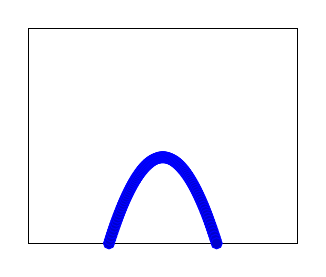
\begin{tikzpicture}
			\begin{axis}[
					width=5cm,
					xmin=-5,xmax=5,
					xmin=-5,xmax=5,
					ymin=-5,ymax=5,
					xtick={-10,...,-9},
					ytick={-10,...,-9},
				]
				\addplot expression[domain=-2:2,samples=100]{-1*x^2-1};
			\end{axis}
		\end{tikzpicture}
	\end{adjustbox}
	& 
	$b^2-4ac<0$ 
	\begin{itemize}
		\item {\em no} real solutions
		\item the graph does {\em not} touch the horizontal axis at all
	\end{itemize} \\ 
\end{longtable}

We study each of the 3 cases in the following examples. 

\begin{myexample}
State the coordinates of the horizontal intercepts (as ordered pairs) for each of the given quadratic functions.
\end{myexample}

\begin{minipage}{.5\textwidth}
	\begin{tikzpicture}
		\begin{axis}[
				framed,
				xmin=-5,xmax=5,
				ymin=-5,ymax=5,
				xtick={-4,...,4},
				ytick={-4,...,4},
				grid=major,
				width=\textwidth,
			]
			\addplot expression[domain=-2.23:2.23,samples=100]{x^2-1};
			\addplot[cmhplot,soldot]coordinates{	(1,0) (-1,0) 	};
		\end{axis}
	\end{tikzpicture}
\end{minipage}%
\hfill
\begin{minipage}{.4\textwidth}
	$f(x)=x^2-1$
	
	$x$-intercepts: $(1,0)$, $(-1,0)$
	
	$a>0$, and the parabola opens upwards.
\end{minipage}%

\begin{minipage}{.5\textwidth}
	\begin{tikzpicture}
		\begin{axis}[
				framed,
				xmin=-5,xmax=5,
				ymin=-5,ymax=5,
				xtick={-4,...,4},
				ytick={-4,...,4},
				grid=major,
				width=\textwidth,
			]
			\addplot expression[domain=-2:4,samples=100]{(x-3)*(x+1)};
			\addplot[cmhplot,soldot] 	coordinates{	(3,0) 	(-1,0) 	};
		\end{axis}
	\end{tikzpicture}
\end{minipage}%
\hfill
\begin{minipage}{.4\textwidth}
	$f(x)=(x-3)(x+1)$
	    
	$x$-intercepts: $(3,0)$, $(-1,0)$
	
	$a>0$ and the parabola opens upwards.
\end{minipage}%

\begin{minipage}{.5\textwidth}
	\begin{tikzpicture}
		\begin{axis}[
				framed,
				xmin=-5,xmax=5,
				ymin=-5,ymax=5,
				xtick={-4,...,4},
				ytick={-4,...,4},
				grid=major,
				width=\textwidth,
			]
			\addplot expression[domain=-0.75:3.8,samples=100]{-1*(x-2)*(x-1)};
			\addplot[cmhplot,soldot] coordinates{	(2,0) (1,0) 	};
		\end{axis}
	\end{tikzpicture}
\end{minipage}%
\hfill
\begin{minipage}{.4\textwidth}
	$f(x)=-(x-2)(x-1)$
	    
	$x$-intercepts: $(2,0)$, $(1,0)$
	
	$a<0$ and the parabola opens upwards.
\end{minipage}%

\begin{minipage}{.5\textwidth}
	\begin{tikzpicture}
		\begin{axis}[
				framed,
				xmin=-5,xmax=5,
				ymin=-5,ymax=5,
				xtick={-4,...,4},
				ytick={-4,...,4},
				grid=major,
				width=\textwidth,
			]
			\addplot expression[domain=-0.25:4,samples=100]{-1*(x-2)^2};
			\addplot[cmhplot,soldot] coordinates{	(2,0) };
		\end{axis}
	\end{tikzpicture}
\end{minipage}%
\hfill
\begin{minipage}{.4\textwidth}
	$f(x)=-(x-2)^2$
	
	$x$-\gls{intercept}: $(2,0)$
	
	$a<0$ and the parabola opens downwards.
\end{minipage}%

\begin{minipage}{.5\textwidth}
	\begin{tikzpicture}
		\begin{axis}[
				framed,
				xmin=-5,xmax=5,
				ymin=-5,ymax=5,
				xtick={-4,...,4},
				ytick={-4,...,4},
				grid=major,
				width=\textwidth,
			]
			\addplot expression[domain=-4.75:-1,samples=100]{(x+3)^2+1};
		\end{axis}
	\end{tikzpicture}
\end{minipage}%
\hfill
\begin{minipage}{.4\textwidth}
	$f(x)=(x+3)^2+1$
	
	$x$-intercepts: none
	
	$a>0$ and the parabola opens upwards.
\end{minipage}


\begin{myexample}\label{ex:horizints1}
Find the $x$ intercepts of 
\[
	f(x) = x^2-9
\]
and state your answers as ordered pairs.
\end{myexample}
\begin{myProof}
	The $x$ intercepts are when $y=0$, so we have to \gls{solve} the equation
	\[
		0 = x^2-9
	\]
	We have studied this example previously (see \vref{ex:quadform1}) and know
	that the solutions are 
	\[
		x = \pm 3
	\]
	The horizontal intercepts of the given function are therefore
	\[
		(3,0), \qquad (-3,0)
	\]
	This is seen in \cref{fig:quad}; note in particular that the horizontal intercepts
	are shown with bullets.
			
	\begin{figure}[!ht]
		\centering
		\begin{tikzpicture}
			\begin{axis}[
					framed,
					xmin=-10,xmax=10,
					ymin=-10,ymax=10,
					xtick={-8,-6,...,8},
					minor xtick={-9,-7,...,9},
					ytick={-8,-6,...,8},
					minor ytick={-9,-7,...,9},
					grid=both,
					legend pos=south east,
				]
				\addplot expression[domain=-4.1:4.1,samples=100]{x^2-9};
				\addplot[cmhplot,soldot] coordinates{	(3,0) (-3,0) };
				\legend{$f(x)=x^2-9$};
			\end{axis}
		\end{tikzpicture}
		\caption{The quadratic function $f(x)=x^2-9$; note that there are 2 real solutions.}
		\label{fig:quad}
	\end{figure}
			
\end{myProof}


\begin{myexample}\label{ex:horizints2}
Find the $x$ intercepts of 
\[
	f(x) = x^2+2x+1
\]
and state your answers as ordered pairs.

\end{myexample}
\begin{myProof}
	We need to solve the equation
	\[
		0 = x^2+2x+1
	\]
	which we can do using any of the methods discussed so far. On factoring this \gls{expression} we obtain
	\[
		(x+1)^2=0
	\]
	and therefore $x=-1$ twice. We conclude that there is only one horizontal intercept, and it is at
	\[
		(-1,0)
	\]
	As there is only one $x$ intercept, the curve {\em touches} the horizontal axis at this \gls{point}, as shown 
	in \cref{fig:quad1}.
	\begin{figure}[!ht]
		\centering
		\begin{tikzpicture}
			\begin{axis}[
					framed,
					xmin=-10,xmax=10,
					ymin=-10,ymax=10,
					xtick={-8,-6,...,8},
					minor xtick={-9,-7,...,9},
					ytick={-8,-6,...,8},
					minor ytick={-9,-7,...,9},
					grid=both,
					legend pos=south east,
				]
				\addplot expression[domain=-4:2,samples=100]{x^2+2*x+1};
				\addplot[cmhplot,soldot] coordinates{	(-1,0) };
				\legend{$f(x)=x^2+2x+1$};
			\end{axis}
		\end{tikzpicture}
		\caption{The quadratic function $f(x)=x^2+2x+1$; note that there is only one horizontal intercept, which is located at $(-1,0)$.}
		\label{fig:quad1}
	\end{figure}
	{}
\end{myProof}

\FloatBarrier

\begin{myexample}\label{ex:horizints3}
Find the $x$ intercepts of 
\[
	f(x) = -x^2-2x-4
\]
and state your answers as an ordered pair.
\end{myexample}
\begin{myProof}
	As in the previous examples, to find the horizontal intercepts we need to set the function equal to zero. 
	We therefore need to solve the equation
	\begin{equation}\label{equn:norealsolns}
		0 = -x^2-2x-4
	\end{equation}
	We can solve this equation using any of the techniques that we have discussed so far. It does not
	\gls{factor}, so let's use the quadratic formula
	\begin{align*}
		x & =   \frac{-b\pm \sqrt{b^2-4ac}}{2a}                \\
		  & =   \frac{-(-2)\pm \sqrt{(-2)^2-4(-1)(-4)}}{2(-1)} \\
		  & =  \frac{2\pm\sqrt{4-16}}{-2}                      \\
		  & =  \frac{2\pm \sqrt{-12}}{-2}                      
	\end{align*} 
	{}
	Notice that we have an expression that contains the square root of a negative number, which is not real. 
	We therefore conclude that there are no real solutions to \cref{equn:norealsolns}, and there
	are no horizontal intercepts. This is shown graphically in \cref{fig:quad2}.
			
	\begin{figure}[!ht]
		\centering
		\begin{tikzpicture}
			\begin{axis}[
					framed,
					xmin=-10,xmax=10,
					ymin=-10,ymax=10,
					xtick={-8,-6,...,8},
					minor xtick={-9,-7,...,9},
					ytick={-8,-6,...,8},
					minor ytick={-9,-7,...,9},
					grid=both,
				]
				\addplot expression[domain=-3.4:1.5,samples=100]{-1*x^2-2*x-4};
				\legend{$f(x)=-x^2-2x-4$};
			\end{axis}
		\end{tikzpicture}
		\caption{The quadratic function $f(x)=-x^2-2x-4$; note that there are no horizontal intercepts.}
		\label{fig:quad2}
	\end{figure}
	{}
	\FloatBarrier
\end{myProof}


\subsection{Vertical intercept}
The vertical intercept is the point where the curve cuts the vertical axis. All quadratic functions have a vertical
intercept, and we find it by evaluating $f(0)$.

\begin{myexample}
Find the vertical intercept of
\[
	f(x) = x^2-x+6
\]
{}
\end{myexample}
\begin{myProof}
	We set $x=0$, and obtain
	\begin{align*}
		f(0) & =   (0)^2-0+6 \\
		     & =  6          \\
	\end{align*} 
	The vertical intercept of this function is at $(0,6)$; see \cref{fig:quad3}.
	\begin{figure}[!ht]
		\centering
		\begin{tikzpicture}
			\begin{axis}[
					framed,
					xmin=-5,xmax=5,
					ymin=-2,ymax=20,
					grid=major,
					xtick={-4,...,4},
					ytick={2,4,...,18},
				]
				\addplot expression[domain=-3.27:4.27,samples=100]{x^2-x+6};
				\addplot[cmhplot,soldot] coordinates{	(0,6) };
				\legend{$f(x)=x^2-x+6$};
			\end{axis}
		\end{tikzpicture}
		\caption{The quadratic function $f(x)=x^2-x+6$; note the vertical intercept at $(0,6)$. }
		\label{fig:quad3}
	\end{figure}
	\FloatBarrier
			
\end{myProof} 

\begin{myexample}
Find the vertical intercepts for \cref{ex:horizints1,ex:horizints2,ex:horizints3}
\end{myexample}
\begin{myProof}
	See if you can do this question on your own first! 
			
	The solutions are shown in the footnote\footnote{\cref{ex:horizints1}: $(0,9)$, \cref{ex:horizints2}:$(0,1)$, \cref{ex:horizints3}:$(0,-4)$}. 
\end{myProof}


\subsection{\Gls{vertex} coordinates}
Every quadratic has a vertex and an axis of symmetry. The vertex is the turning point of the parabola, and the axis of symmetry
is the line about which the graph is symmetric. Some examples are shown in \cref{fig:vertexdemo}.

\begin{figure}[ht]
	\begin{subfigure}{.45\textwidth}
		\centering
		\begin{tikzpicture}
			\begin{axis}[
					framed,
					width=\textwidth,
					xmin=-5,xmax=5,
					ymin=-5,ymax=5,
					xtick={-4,-2,...,4},
					ytick={-4,-2,...,4},
					minor xtick={-3,-1,...,3},
					minor ytick={-3,-1,...,3},
					grid=both,
				]
				\addplot expression[domain=-0.5:4.5,samples=100]{(x-2)^2-3};
				\addplot[cmhplot,soldot] coordinates{	(2,-3) 	};
			\end{axis}
		\end{tikzpicture}
		\caption{$a>0$: Vertex is at $(2,-3)$}
	\end{subfigure}%
	\hfill
	\begin{subfigure}{.45\textwidth}
		\centering
		\begin{tikzpicture}
			\begin{axis}[
					framed,
					width=\textwidth,
					xmin=-5,xmax=5,
					ymin=-5,ymax=5,
					xtick={-4,-2,...,4},
					minor xtick={-3,-1,...,3},
					minor ytick={-3,-1,...,3},
					ytick={-4,-2,...,4},
					grid=both,
				]
				\addplot expression[domain=-0.5:4.5,samples=100]{-1*(x-2)^2+3};
				\addplot[cmhplot,soldot] coordinates{	(2,3) };
			\end{axis}
		\end{tikzpicture}
		\caption{$a<0$: Vertex is at $(2,3)$}
	\end{subfigure}
	\caption{Notice that when $a>0$ the vertex is the lowest point on the parabola
	and when $a<0$ the vertex is the highest point on the parabola}
	\label{fig:vertexdemo}
\end{figure}

We can find the $x$ coordinate of the vertex of any quadratic using the formula
\[
	x = - \frac{b}{2a}
\]	
and the vertical coordinate is found by substituting this value in for $x$; we demonstrate
this with examples. 

\begin{myexample}
Find the coordinates of the vertex of
\begin{equation}\label{equn:vertex1}
	f(x) = x^2+x+5
\end{equation}
{}
\end{myexample}
\begin{myProof}
	We use the formula given above to find the $x$ coordinate of the vertex
	\begin{align*}
		x & =  - \frac{b}{2a}   \\
		  & =  - \frac{1}{2(1)} \\
		  & =  -\frac{1}{2}     
	\end{align*} 
	We find the $y$ coordinate by substituting this value of $x$ into \cref{equn:vertex1}
	\begin{align*}
		f\left(-\frac{b}{2a}\right) & =  \left(-\frac{1}{2}\right)^2 +\left(- \frac{1}{2}\right)+5 \\
		                            & =  \frac{1}{4}-\frac{1}{2}+5                                 \\
		                            & =  \frac{19}{4}                                              
	\end{align*} 
	Therefore, the coordinates of the vertex of this quadratic function are 
	\[
		\left( -\frac{1}{2}, \frac{19}{4}\right)
	\]
	which is shown in \cref{fig:quadvertex1}.
			
	\begin{figure}[!ht]
		\centering
		\begin{tikzpicture}
			\begin{axis}[
					framed,
					xmin=-5,xmax=5,
					ymin=-5,ymax=20,
					xtick={-4,...,4},
					ytick={-4,-2,...,18},
					grid=major,
				]
				\addplot expression[domain=-4.405:3.405,samples=100]{x^2+x+5};
				\addplot[cmhplot,soldot] coordinates{	(-0.5,4.75)	};
				\legend{$f(x)=x^2+x+5$};
			\end{axis}
		\end{tikzpicture}
		\caption{The quadratic function $f(x)=x^2+x+5$; notice that we have marked the vertex $\left(-\frac{1}{2}, \frac{19}{4}\right)$.}
		\label{fig:quadvertex1}
	\end{figure}
\end{myProof}

\FloatBarrier

\begin{myexample}
Find the coordinates of the vertex of
\[
	f(x) = -x^2 - 3x -4
\]
and state your answer as an ordered pair.
\end{myexample}
\begin{myProof}
	We follow the same procedure as illustrated previously, and begin by finding
	the $x$ coordinate
	\begin{align*}
		x & =  -\frac{b}{2a}     \\
		  & =  -\frac{-3}{2(-1)} \\
		  & =  -\frac{3}{2}      
	\end{align*} 
	The $y$ coordinate can be found by substituting this value of $x$ into the original
	quadratic function
	\begin{align*}
		f\left(-\frac{b}{2a}\right) & =  - \left(-\frac{3}{2}\right)^2 - 3\left(- \frac{3}{2}\right)-4 \\
		                            & =  -\frac{9}{4}+\frac{9}{2} - 4                                  \\
		                            & =  - \frac{7}{4}                                                 
	\end{align*} 
	This can be seen in \cref{fig:quadvertex2}.
			
	\begin{figure}[!ht]
		\centering
		\begin{tikzpicture}
			\begin{axis}[
					framed,
					xmin=-5,xmax=5,
					ymin=-10,ymax=5,
					xtick={-4,...,4},
					ytick={-9,...,4},
					grid=major,
				]
				\addplot expression[domain=-4.37:1.37,samples=100]{-1*x^2-3*x-4};
				\addplot[cmhplot,soldot]coordinates{	(-1.5,-1.75) 	};
				\legend{$f(x)=-x^2-3x-4$};
			\end{axis}
		\end{tikzpicture}
		\caption{The quadratic function $f(x)=-x^2-3x-4$; note that we have marked the vertex.}
		\label{fig:quadvertex2}
	\end{figure}
	\FloatBarrier
\end{myProof} 

\subsection{Plotting a quadratic function}
We now combine all of these ideas and plot a quadratic. We will find all of the features we have just 
described, together with at least 3 ordered pairs in order to help us plot an accurate graph. 

Note: the example given here will be plotted using a computer package, but it is intended that you perform
the exercises {by hand on graphing paper}.

\begin{myexample}
Plot the quadratic function
\[
	f(x) = x^2+2x-3
\]
{}
\end{myexample}
\begin{myProof}
	Note first of all that $a=1>0$, we therefore know that the graph will be a parabola that opens
	upwards.
			
	Our approach will be to find
	\begin{itemize}
		\item $x$ intercepts (if any):\\
		We find the $x$ intercepts by solving the equation
		\[
			x^2+2x-3=0
		\]
		At this stage our factoring skills should be suitable sharp that we can spot that this quadratic
		can be factored to
		\[
			(x+3)(x-1)=0
		\]
		and therefore $x=-3$ or $x=1$. This means that the $x$ intercepts are at 
		\[
			(-3,0), \qquad and \qquad (1,0)
		\]
		\item $y$ intercept:\\
		We find this by evaluating $f(0)$, and therefore
		\begin{align*}
			f(0) & =  0^2+2(0)-3 \\
			     & =  -3         
		\end{align*} 
		The vertical intercept is at $(0,-3)$.
		\item coordinates of the vertex:\\
		The $x$ coordinate of the vertex is
		\begin{align*}
			x & =  - \frac{b}{2a}   \\
			  & =  - \frac{2}{2(1)} \\
			  & =  - 1              
		\end{align*} 
		The $y$ coordinate of the vertex is 
		\begin{align*}
			f(-1) & =  (-1)^2+2(-1)-3 \\
			      & =  -4             
		\end{align*} 
		The coordinates of the vertex are $(-1,-4)$.
		\item three other ordered pairs:\\
		We can choose any $x$ values we wish, but it makes sense to try and choose them close to the points that 
		we have already
		\begin{center}
			\begin{tabular}{SS}
				\toprule
				{$x$} & {$y$} \\
				\midrule
				-4    & 5     \\
				-2    & -3    \\
				2     & 5     \\
				\bottomrule
			\end{tabular} 
		\end{center}
	\end{itemize}
	We now plot these points on a graph, see \cref{fig:plotpointsquad}.
			
	\tikzstyle{every pin}=[fill=white, draw=blue]
	\begin{figure}[!ht]
		\centering
		\begin{tikzpicture}
			\begin{axis}[
					framed,
					xmin=-10,xmax=10,
					ymin=-10,ymax=10,
					xtick={-8,-6,...,8},
					ytick={-8,-6,...,8},
					minor xtick={-9,-7,...,9},
					minor ytick={-9,-7,...,9},
					grid=both,
				]
				\node[coordinate,pin=left:{\tiny Vertex}]at (axis cs:-1,-4) {};
				\node[coordinate,pin=right:{\tiny Vertical Intercept}]at (axis cs:0,-3) {};
				\node[coordinate,pin=left:{\tiny Horizontal Intercept}]at (axis cs:-3,0) {};
				\node[coordinate,pin=right:{\tiny Horizontal Intercept}]at (axis cs:1,0) {};
				\addplot[cmhplot,soldot] coordinates{	(-4,5)(-3,0)(-2,-3)(-1,-4)(0,-3)(1,0)(2,5)};
			\end{axis}
		\end{tikzpicture}
		\caption{We begin by plotting the ordered pairs.}
		\label{fig:plotpointsquad}
	\end{figure}
	\FloatBarrier
			
	Once we have drawn the points, we can connect them together as a smooth curve (\cref{fig:connected}).
			
	\begin{figure}[!ht]
		\centering
		\begin{tikzpicture}
			\centering
			\begin{axis}[
					framed,
					xmin=-10,xmax=10,
					ymin=-10,ymax=10,
					xtick={-8,-6,...,8},
					ytick={-8,-6,...,8},
					minor xtick={-9,-7,...,9},
					minor ytick={-9,-7,...,9},
					grid=both,
					legend pos=south west,
				]
				\addplot expression[domain=-4.5:2.7,samples=100]{x^2+2*x-3};
				\addplot[cmhplot,soldot] coordinates{	(-4,5)(-3,0)(-2,-3)(-1,-4)(0,-3)(1,0)(2,5)};
				\legend{$f(x)=x^2+2x-3$};
			\end{axis}
		\end{tikzpicture}
		\caption{Now connect all of the points using a smooth curve.}
		\label{fig:connected}
	\end{figure}
	\FloatBarrier
			
\end{myProof} 


\pgfplotsset{every axis/.append style={width=8cm}}

\begin{myexample}
Match each of the following quadratic functions with one of the graphs 
below.
\begin{multicols}{2}
	\begin{itemize}
		\item $f(x)=-x^2$
		\item $f(x)=(x+3)(x-1)$
		\item $f(x)=-(x+2)^2$
		\item $f(x)=(x+2)(x-1)$
	\end{itemize}
\end{multicols}
\end{myexample}


\begin{minipage}{.5\textwidth}
	\begin{tikzpicture}
		\begin{axis}[
				framed,
				xmin=-5,xmax=5,
				ymin=-5,ymax=5,
				grid=major,
				xtick={-4,...,4},
				ytick={-4,...,4}
			]
			\addplot expression[domain=-4:2,samples=100]{(x+3)*(x-1)};
		\end{axis}
	\end{tikzpicture}
\end{minipage}%
\hfill
\begin{minipage}{.4\textwidth}
	$f(x)=$\solution{$(x+3)(x-1)$}
			
	$x$ intercepts: \solution{$\{(-3,0),(1,0)\}$}
			
	$y$ intercept:  \solution{$(0,-3)$}
			
	axis of symmetry:  \solution{$x=-1$}
			
	vertex:  \solution{$(-1,-4)$}
\end{minipage}

\begin{minipage}{.5\textwidth}
	\begin{tikzpicture}
		\begin{axis}[
				framed,
				xmin=-5,xmax=5,
				ymin=-5,ymax=5,
				grid=major,
				xtick={-4,...,4},
				ytick={-4,...,4}
			]
			\addplot expression[domain=-2.1:2.1,samples=100]{-1*x^2};
		\end{axis}
	\end{tikzpicture}
\end{minipage}%
\hfill
\begin{minipage}{.4\textwidth}
	$f(x)=$ \solution{$-x^2$}
			
	$x$ intercepts:  \solution{$(0,0)$}
			
	$y$ intercept:  \solution{$(0,0)$}
			
	axis of symmetry:  \solution{$x=0$}
			
	vertex:  \solution{$(0,0)$}\
\end{minipage}

\begin{minipage}{.5\textwidth}
	\begin{tikzpicture}
		\begin{axis}[
				framed,
				xmin=-5,xmax=5,
				ymin=-5,ymax=5,
				grid=major,
				xtick={-4,...,4},
				ytick={-4,...,4}
			]
			\addplot expression[domain=-3.1:2.1,samples=100]{-(x+2)*(x-1)};
		\end{axis}
	\end{tikzpicture}
\end{minipage}%
\hfill
\begin{minipage}{.4\textwidth}
	$f(x)=$ \solution{$(x+2)(x-1)$}
			
	$x$ intercepts:  \solution{$(-2,0),(1,0)$}
			
	$y$ intercept:  \solution{$(0,-2)$}
			
	axis of symmetry:  \solution{$x=-\frac{1}{2}$}
			
	vertex:  \solution{$\left(-\frac{1}{2}, -\frac{9}{4}\right)$}
\end{minipage}

\begin{minipage}{.5\textwidth}
	\begin{tikzpicture}
		\begin{axis}[
				framed,
				xmin=-5,xmax=5,
				ymin=-5,ymax=5,
				grid=major,
				xtick={-4,...,4},
				ytick={-4,...,4},
				width=\textwidth,
			]
			\addplot expression[domain=-4.1:1.01,samples=100]{-1*(x+2)^2};
		\end{axis}
	\end{tikzpicture}
\end{minipage}%
\hfill
\begin{minipage}{.4\textwidth}
	$f(x)=$ \solution{$-(x+2)^2$}
			
	$x$ intercepts:  \solution{$(-2,0)$}
			
	$y$ intercept:  \solution{$(0,-4)$}
			
	axis of symmetry:  \solution{$x=-2$}
			
	vertex:  \solution{$(-2,0)$}
\end{minipage}

\begin{myexample}
\drillandskill
Give a possible formula for a quadratic function that has zeros at
\begin{enumerate}
	\item $x=1,2$ \solution{$f(x)=(x-1)(x-2)$}
	\item $x=-1,1$ \solution{$f(x)=(x+1)(x-1)$} 
	\item $x=0,3$ \solution{$f(x)=x(x-3)$}
	\item $x=-3,4$ \solution{$f(x)=(x+3)(x-4)$}
\end{enumerate}
\end{myexample}

\subsection{Summary of plotting a quadratic}
When plotting a quadratic there are four main tasks:
\begin{itemize}
	\item decide if the graph opens upward ($a>0$) or downward ($a<0$)
	\item find the $x$ intercepts by setting $y=0$
	\item find the vertical intercept by setting $x=0$
	\item find the coordinates of the vertex
\end{itemize} 
We should also find three additional points so that we can draw a smooth curve. 
